%% Single Figure Environment
\documentclass[12pt]{article}
\usepackage{graphicx}
\graphicspath{{Images/}} %% Path to find Image Files
\usepackage{caption} %% For using Sub-Figure and Sub-Table Environments
\usepackage{subcaption}


\usepackage{float}
\usepackage[section]{placeins} % \FloatBarrier, it avoids floating of tables and

\begin{document}

%%Single Figure Environment
\begin{figure}[H]
\centering
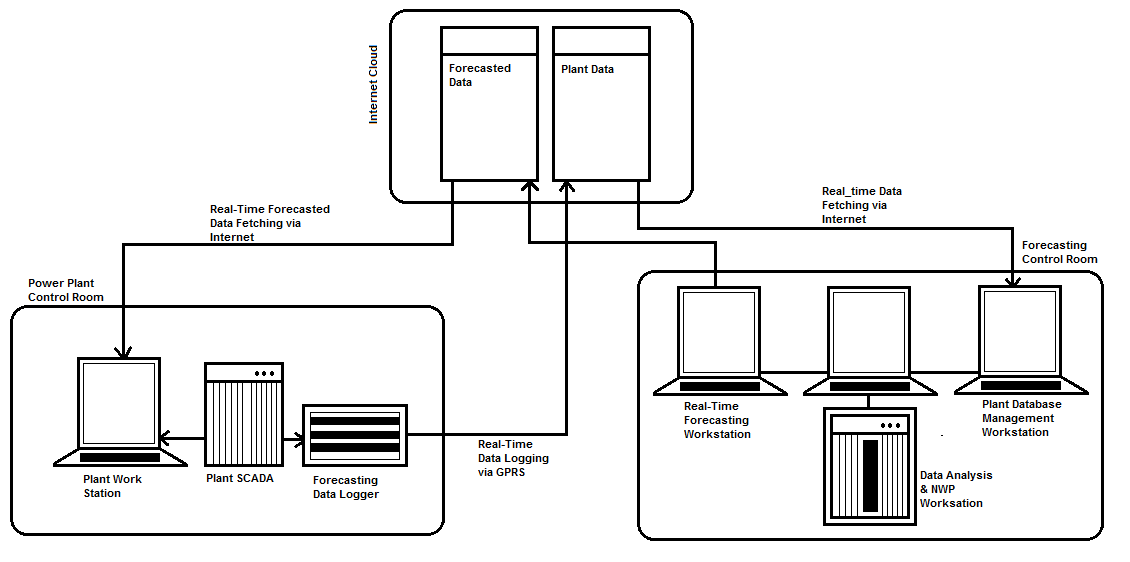
\includegraphics[scale=0.5]{ProposalDesign}
\caption{Future Work - Real-Time Forecasting System}
\label{figc10h1} %% to refer use, \ref{}
\end{figure}

\begin{figure}[H]
\centering
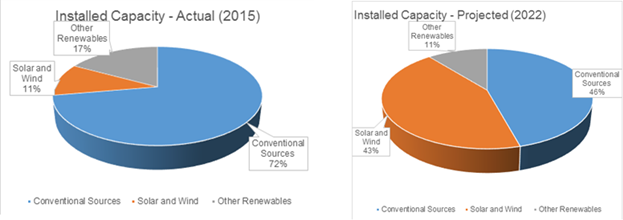
\includegraphics[scale=1]{Intro1}
\caption{Actual and Projected Installed Electricity Generation Capacity Distribution}
\label{figc1h1} %% to refer use, \ref{}
\end{figure}

\begin{figure}[H]
\centering
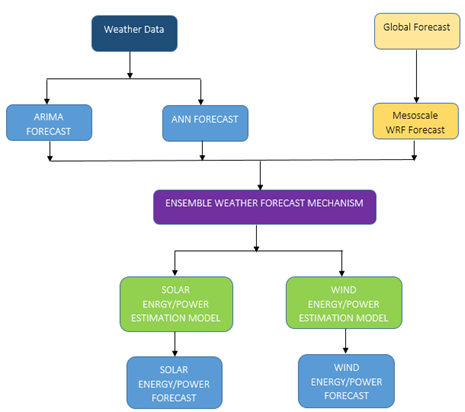
\includegraphics[scale=1]{Intro2}
\caption{Block Diagram – Ensemble Solar/Wind Power Forecasting}
\label{figc1h1} %% to refer use, \ref{}
\end{figure}

\begin{figure}[H]
\centering
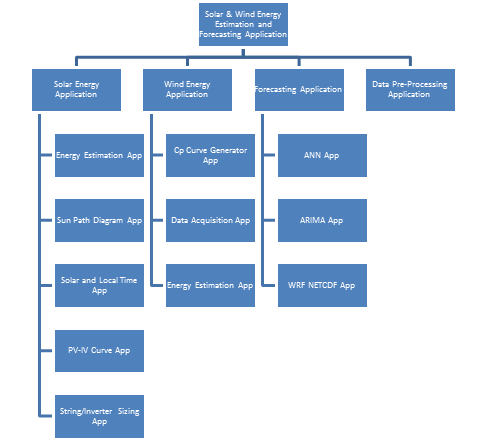
\includegraphics[scale=1]{Intro3}
\caption{Organization of Application}
\label{figc1h1} %% to refer use, \ref{}
\end{figure}


\begin{figure}[H]
\centering
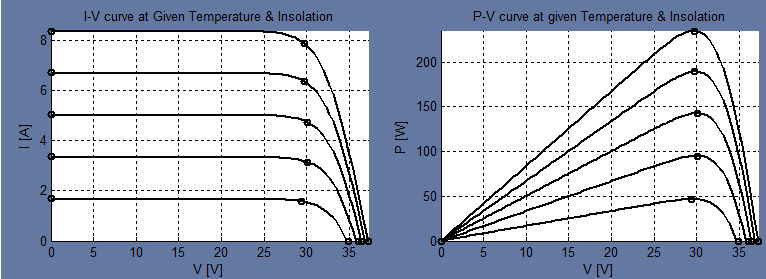
\includegraphics[scale=0.5]{Poly_Irradiance}
\caption{Polycrystalline Solar PV module I-V and P-V Curves at different Irradiances}
\label{figc3h15} %% to refer use, \ref{}
\end{figure}

\begin{figure}[H]
\centering
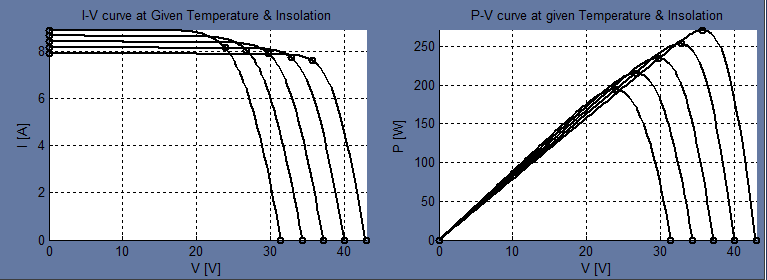
\includegraphics[scale=0.5]{Poly_Temperature}
\caption{Polycrystalline Solar PV module I-V and P-V Curves at different Temperatures}
\label{figc3h16} %% to refer use, \ref{}
\end{figure}

\begin{figure}[H]
\centering
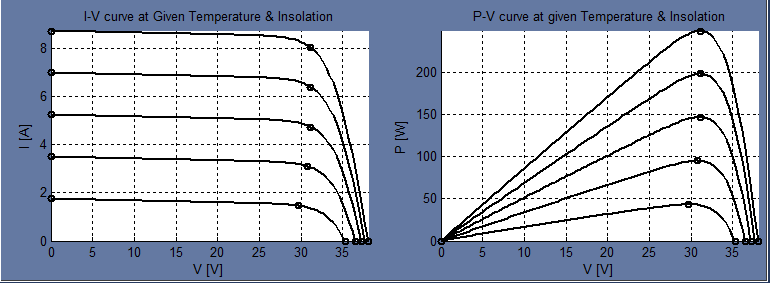
\includegraphics[scale=0.5]{Mono_Irradiance}
\caption{Monocrystalline Solar PV module I-V and P-V Curves at different Irradiances}
\label{figc3h17} %% to refer use, \ref{}
\end{figure}

\begin{figure}[H]
\centering
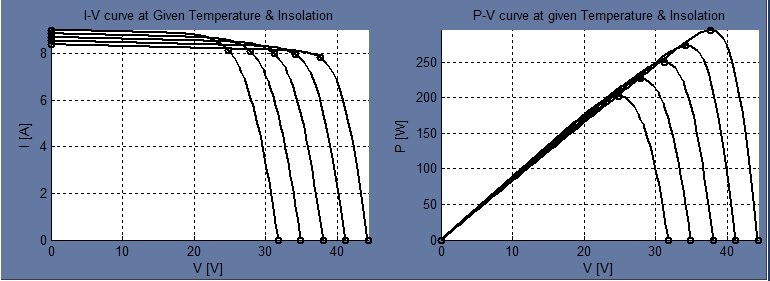
\includegraphics[scale=0.5]{Mono_Temperature}
\caption{Monocrystalline Solar PV module I-V and P-V Curves at different Temperatures}
\label{figc3h18} %% to refer use, \ref{}
\end{figure}

\begin{figure}[H]
\centering
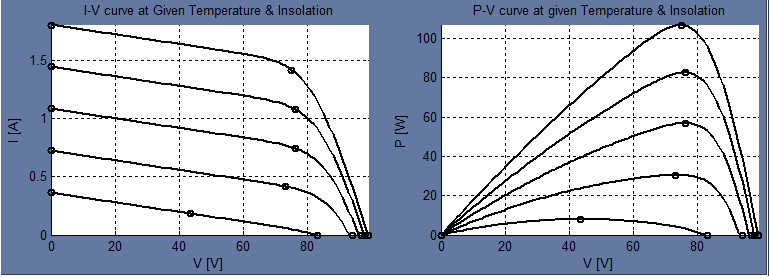
\includegraphics[scale=0.5]{A-si_Irradiance}
\caption{A-Si Thin Film Solar PV module I-V and P-V Curves at different Irradiances}
\label{figc3h19} %% to refer use, \ref{}
\end{figure}

\begin{figure}[H]
\centering
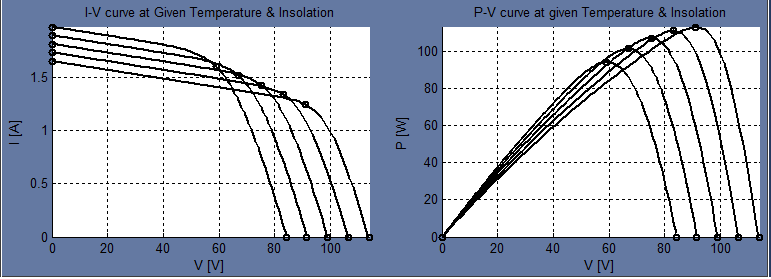
\includegraphics[scale=0.5]{A-si_Temperature}
\caption{A-Si Thin Film Solar PV module I-V and P-V Curves at different Temperatures}
\label{figc3h20} %% to refer use, \ref{}
\end{figure}

\begin{figure}[H]
\centering
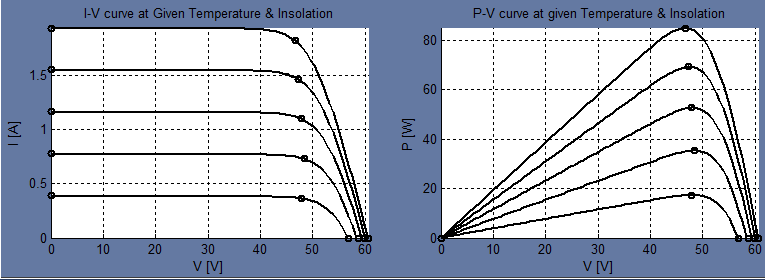
\includegraphics[scale=0.5]{CDTE_Irradiance}
\caption{CDTE Thin Film Solar PV module I-V and P-V Curves at different Irradiances}
\label{figc3h21} %% to refer use, \ref{}
\end{figure}

\begin{figure}[H]
\centering
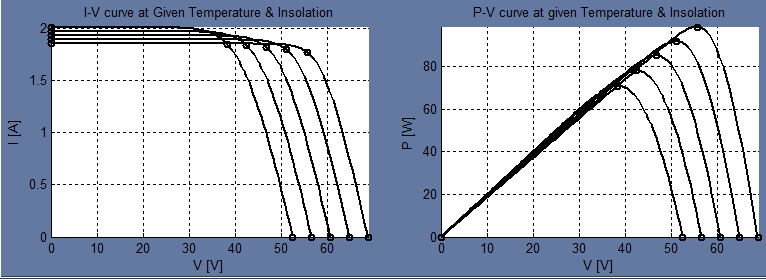
\includegraphics[scale=0.5]{CDTE_Temperature}
\caption{CDTE Thin Film Solar PV module I-V and P-V Curves at different Temperatures}
\label{figc3h22} %% to refer use, \ref{}
\end{figure}

\begin{figure}[H]
\centering
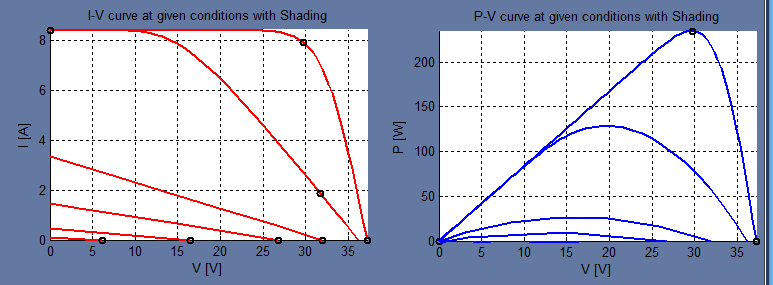
\includegraphics[scale=0.5]{Poly_Shading_WithoutByPassDiode}
\caption{Polycrystalline Solar PV moduleP-V and I-V curves for Shading without Bypass Diode and at different number of shaded cells}
\label{figc3h23} %% to refer use, \ref{}
\end{figure}

\begin{figure}[H]
\centering
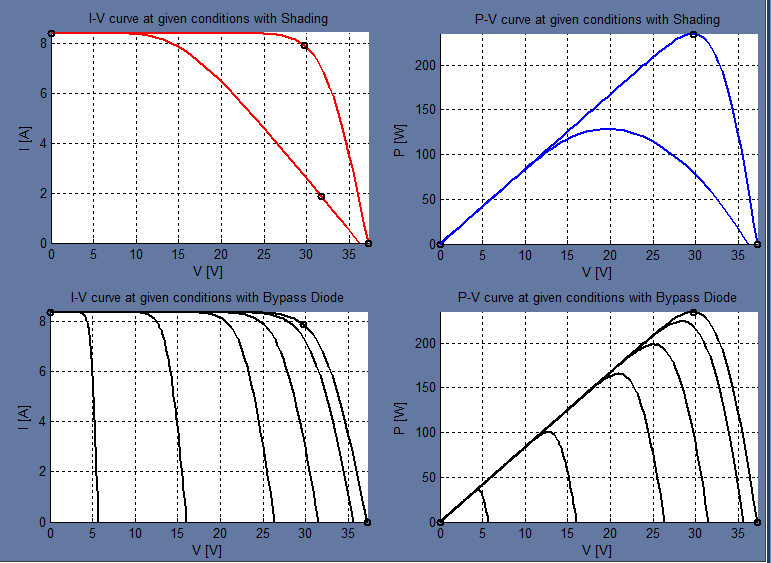
\includegraphics[scale=0.5]{Poly_Shading_With_ByPassDiode}
\caption{Polycrystalline Solar PV moduleP-V and I-V curves for Shading with Bypass Diode and at different number of shaded cells}
\label{figc3h24} %% to refer use, \ref{}
\end{figure}


\begin{figure}[H]
\centering
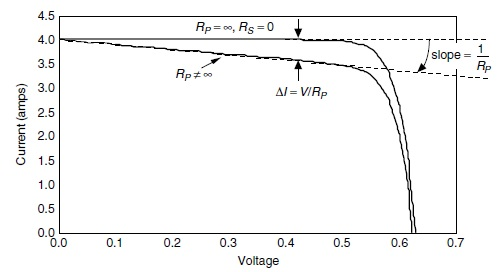
\includegraphics[scale=0.5]{pv1}
\caption{Effect of Parallel Resistance on I-V Curve}
\label{figc3h111} %% to refer use, \ref{}
\end{figure}

\begin{figure}[H]
\centering
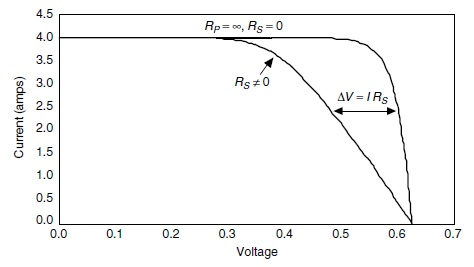
\includegraphics[scale=0.5]{pv2}
\caption{Effect of Series Resistance on I-V Curve}
\label{figc3h222} %% to refer use, \ref{}
\end{figure}

\begin{figure}[H]
\centering
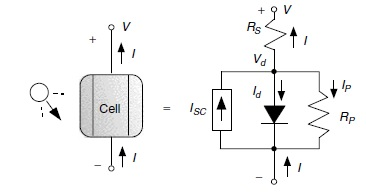
\includegraphics[scale=0.5]{pv3}
\caption{CompleteModel of PV Cell}
\label{figc3h333} %% to refer use, \ref{}
\end{figure}

\begin{figure}[H]
\centering
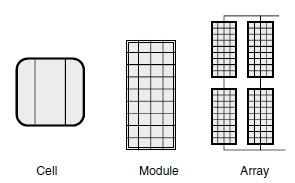
\includegraphics[scale=0.5]{pv4}
\caption{PV - Cell, Module and Array}
\label{figc3h444} %% to refer use, \ref{}
\end{figure}

\begin{figure}[H]
\centering
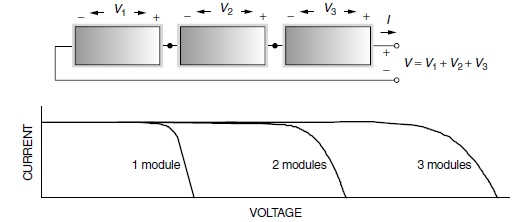
\includegraphics[scale=0.5]{pv5}
\caption{Effect of Series connected modules on I-V Curve}
\label{figc3h555} %% to refer use, \ref{}
\end{figure}

\begin{figure}[H]
\centering
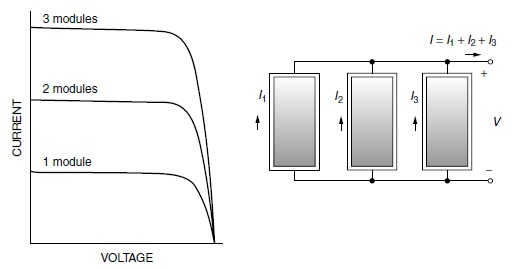
\includegraphics[scale=0.5]{pv6}
\caption{Effect of Parallel connected modules on I-V Curve}
\label{figc3h666} %% to refer use, \ref{}
\end{figure}

\begin{figure}[H]
\centering
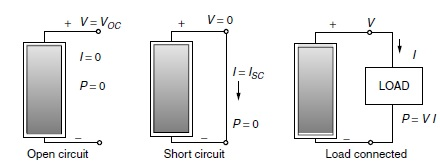
\includegraphics[scale=0.5]{pv7}
\caption{PV module - Open Circuit, Short Circuit and Load Connected}
\label{figc3h777} %% to refer use, \ref{}
\end{figure}

\begin{figure}[H]
\centering
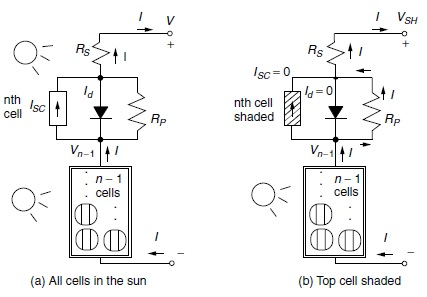
\includegraphics[scale=0.5]{shading1}
\caption{PV module with \textit{n} Cells - top cell in sun, or in shade}
\label{figc3h888} %% to refer use, \ref{}
\end{figure}

\begin{figure}[H]
\centering
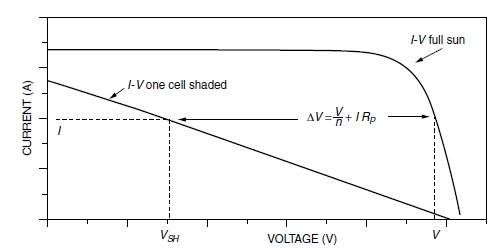
\includegraphics[scale=0.5]{shading2}
\caption{Effect of shading one cell in \textit{n} cell module}
\label{figc3h999} %% to refer use, \ref{}
\end{figure}

\begin{figure}[H]
\centering
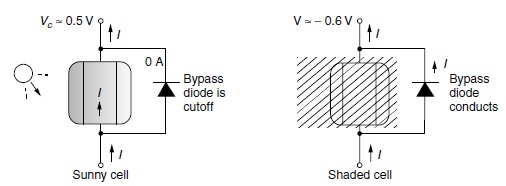
\includegraphics[scale=0.5]{bydiode1}
\caption{Mitigation of shading problem with Bypass Diode - In sunny cell bypass diode is cut-off, in shaded cell it conducts}
\label{figc3h100} %% to refer use, \ref{}
\end{figure}

\begin{figure}[H]
\centering
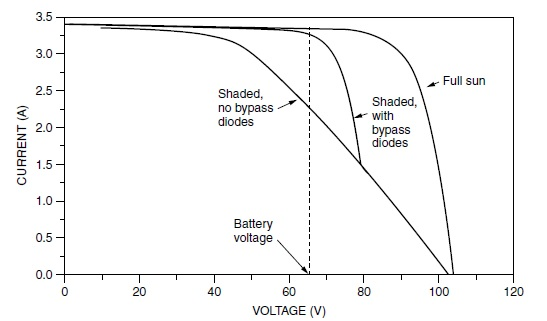
\includegraphics[scale=0.5]{bydiode2}
\caption{Effect of Bypass Diode on I-V Curve}
\label{figc3h190} %% to refer use, \ref{}
\end{figure}

\begin{figure}[H]
\centering
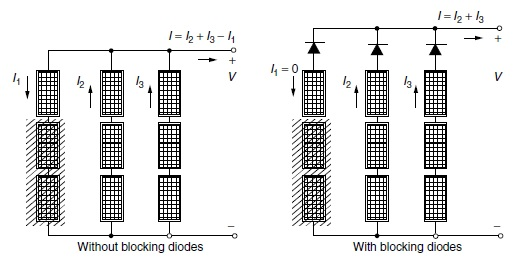
\includegraphics[scale=0.5]{bldiode1}
\caption{Blocking Diode prevents reverse flow of current through PV modules}
\label{figc3h200} %% to refer use, \ref{}
\end{figure}

\begin{figure}[H]
\centering
\includegraphics[scale=0.5]{trac1}
\caption{Charanka Solar Park PV Technology-Wise CUF Comparison}
\label{figc3h17} %% to refer use, \ref{}
\end{figure}

\begin{figure}[H]
\centering
\includegraphics[scale=0.5]{trac2}
\caption{Charanka Solar Park PV Technology-Wise CUF Comparison}
\label{figc3h18} %% to refer use, \ref{}
\end{figure}

\begin{figure}[H]
\centering
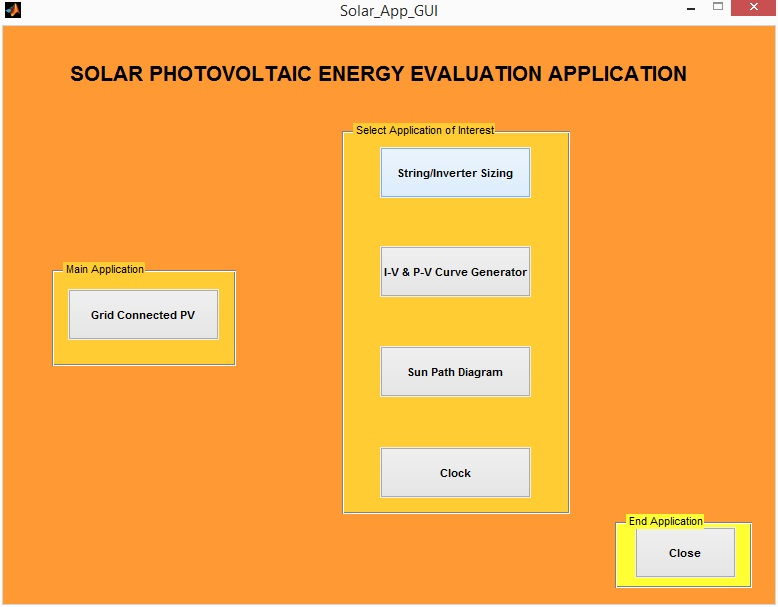
\includegraphics[scale=0.5]{SolarAppGui1}
\caption{Starting Screen of Solar Application}
\label{figApp1_1} %% to refer use, \ref{}
\end{figure}

\begin{figure}[H]
\centering
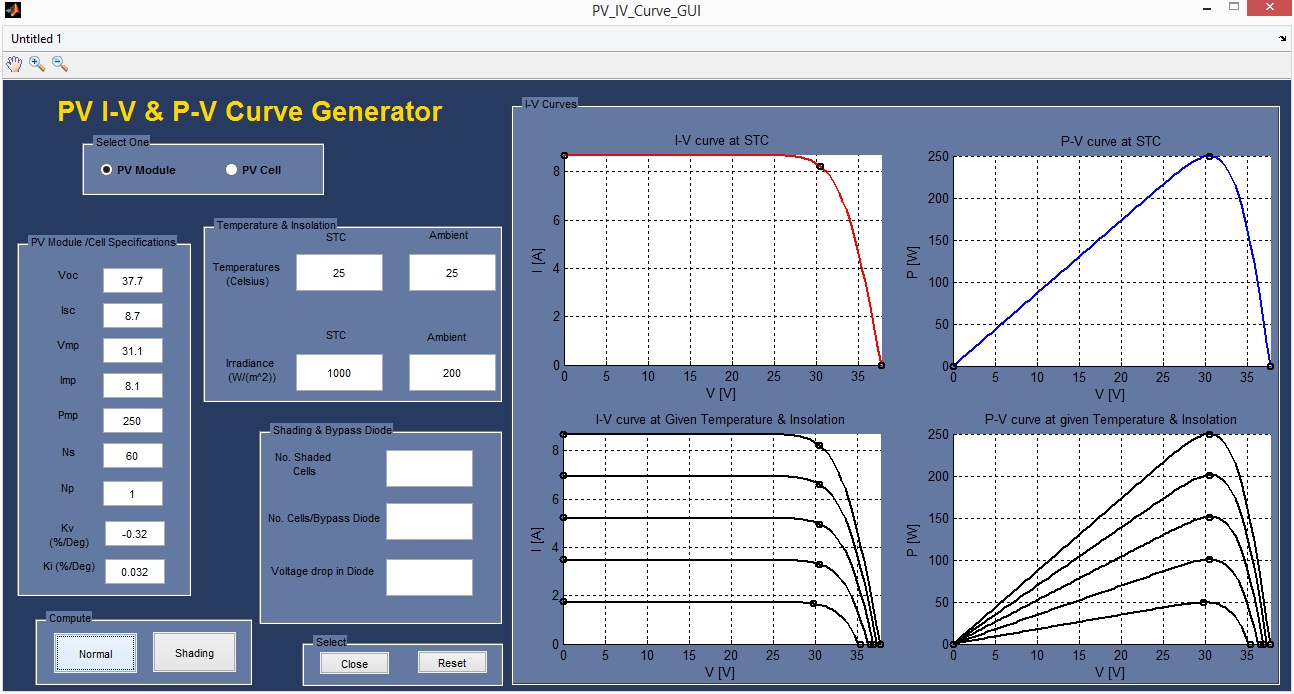
\includegraphics[scale=0.5]{SolarAppGui2}
\caption{PV I-V and P-V Curve Generator Module}
\label{figApp1_2} %% to refer use, \ref{}
\end{figure}

\begin{figure}[H]
\centering
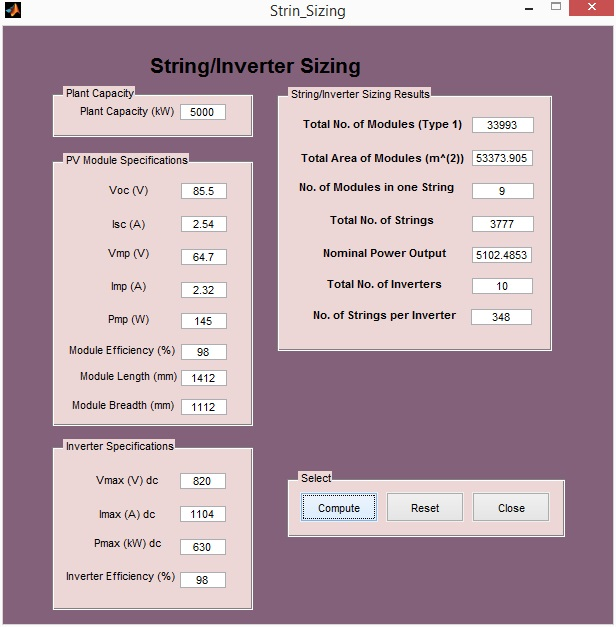
\includegraphics[scale=0.5]{SolarAppGui3}
\caption{String and Inverter Sizing Module}
\label{figApp1_3} %% to refer use, \ref{}
\end{figure}

\begin{figure}[H]
\centering
\includegraphics[scale=0.5]{SolarAppGui8}
\caption{Solar and Regional Clock Module}
\label{figApp1_4} %% to refer use, \ref{}
\end{figure}

\begin{figure}[H]
\centering
\includegraphics[scale=0.5]{SolarAppGui5}
\caption{Grid Connected PV Energy Evaluation Module}
\label{figApp1_5} %% to refer use, \ref{}
\end{figure}

\begin{figure}[H]
\centering
\includegraphics[scale=0.5]{SolarAppGui4}
\caption{Sun Path Diagram Module}
\label{figApp1_6} %% to refer use, \ref{}
\end{figure}

\begin{figure}[H]
\centering
\includegraphics[scale=0.5]{SolarAppGui7}
\caption{Grid Connected PV Energy Result Screen}
\label{figApp1_6} %% to refer use, \ref{}
\end{figure}

\begin{figure}[H]
\centering
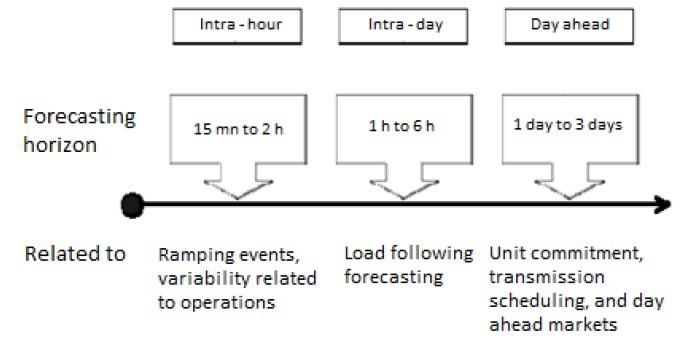
\includegraphics[scale=0.5]{ForecastIntro1}
\caption{Time Horizons for Solar Forecasting}
\label{figc5h1} %% to refer use, \ref{}
\end{figure}

\begin{figure}[H]
\centering
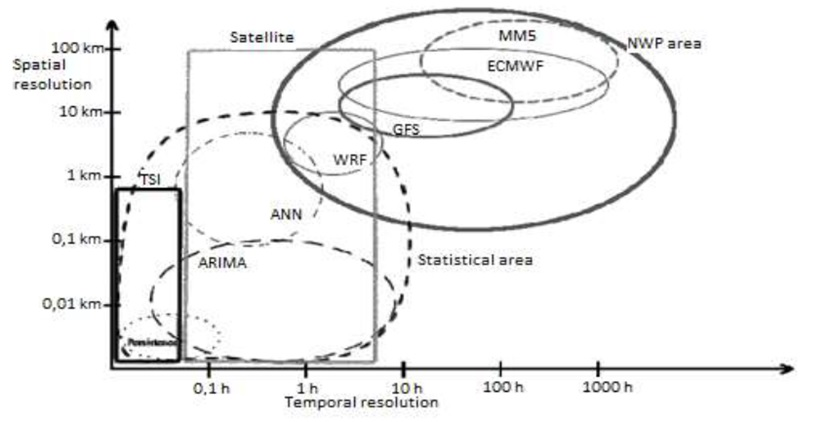
\includegraphics[scale=0.5]{ForecastIntro2}
\caption{Time Horizons for Solar Forecasting}
\label{figc5h1} %% to refer use, \ref{}
\end{figure}

\begin{figure}[H]
\centering
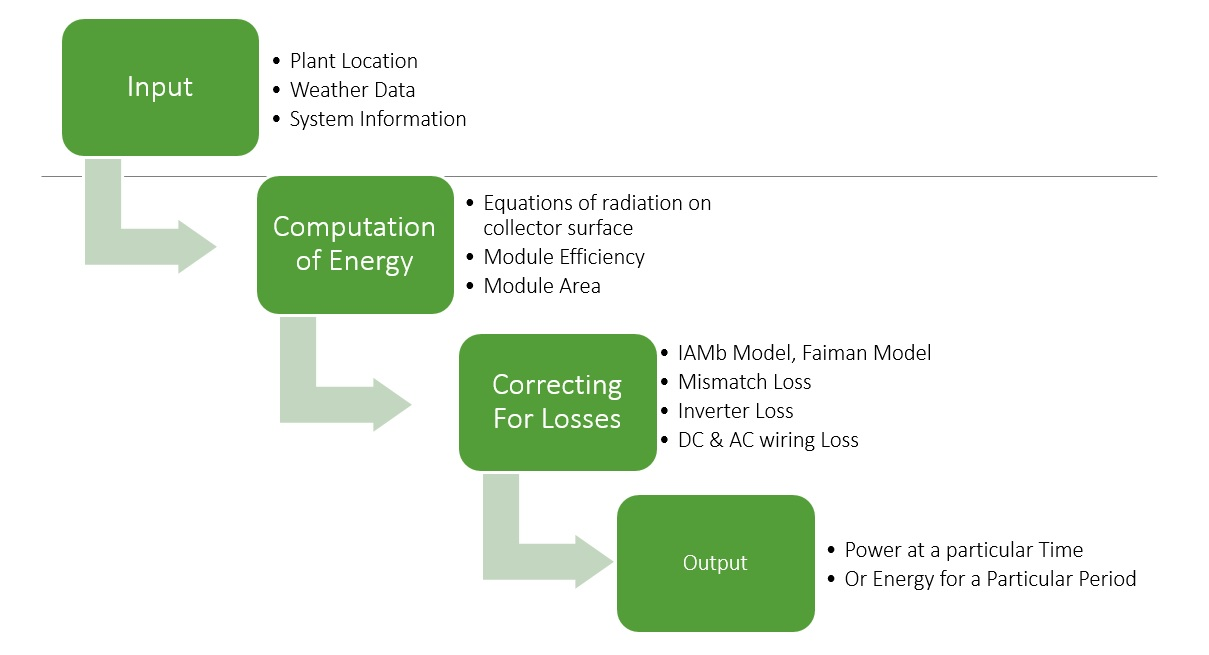
\includegraphics[scale=0.5]{SolarAppAlgorithm}
\caption{Time Horizons for Solar Forecasting}
\label{figc4halgo1} %% to refer use, \ref{}
\end{figure}

\begin{figure}[H]
\centering
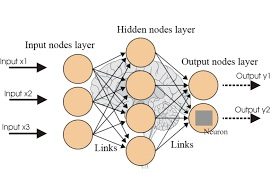
\includegraphics[scale=0.5]{ANN11}
\caption{Feed-Forward Neural Network Schematic}
\label{figc6h3} %% to refer use, \ref{}
\end{figure}

\begin{figure}[H]
\centering
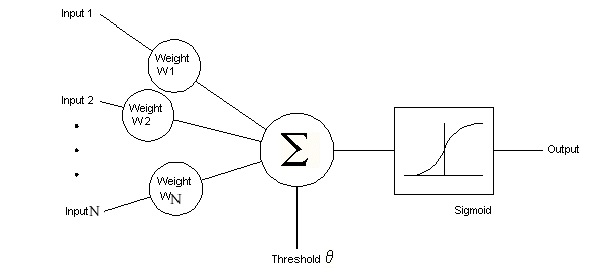
\includegraphics[scale=0.5]{ANN22}
\caption{Artificial Neuron Model}
\label{figc6h4} %% to refer use, \ref{}
\end{figure}

\begin{figure}[H]
\centering
\includegraphics[scale=0.5]{WRF_11}
\caption{WRF Software Schematic}
\label{figc6h5} %% to refer use, \ref{}
\end{figure}

\begin{figure}[H]
\centering
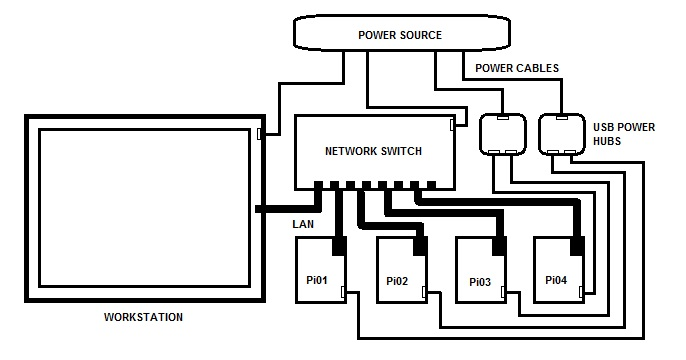
\includegraphics[scale=0.5]{RPiCluster_IMG1}
\caption{Raspberry-Pi Cluster Schematic}
\label{figc6h6} %% to refer use, \ref{}
\end{figure}

\begin{figure}[H]
\centering
\includegraphics[scale=0.5]{Wind11}
\caption{Wind Turbine}
\label{figc5h1} %% to refer use, \ref{}
\end{figure}

\begin{figure}[H]
\centering
\includegraphics[scale=0.5]{Wind2}
\caption{Effect of Altitude on Pressure}
\label{figc5h2} %% to refer use, \ref{}
\end{figure}

\begin{figure}[H]
\centering
\includegraphics[scale=0.5]{Wind3}
\caption{Effect of Hub-Height and Terrain on Wind Velocity}
\label{figc5h3} %% to refer use, \ref{}
\end{figure}

\begin{figure}[H]
\centering
\includegraphics[scale=0.5]{WindScheme}
\caption{Wind Turbine Energy Estimation Schematic}
\label{figc5h4} %% to refer use, \ref{}
\end{figure}

\end{document}